% ************************************************************************
%
% Automated neuron detection in high-content fluorescence microscopy images
% using machine learning 
%
% ************************************************************************
%Automated neuron detection in high-content fluorescence microscopy images using machine learning
\chpos{15mm}{8mm}
\chapter[Automated neuron detection in high-content fluorescence microscopy images using machine learning]{Automated neuron detection in high-content fluorescence microscopy images using machine learning}
\chaptermark{Automated neuron detection in high-content images using machine learning}
\label{ch5:ndetchml}
% abstract
{\small \lettrine{T}{he} study of neuronal morphology in relation to function, and the development of effective medicines to positively impact this relationship in patients suffering from neurodegenerative diseases, increasingly involves image-based high-content screening and analysis. The first critical step toward fully automated high-content image analyses in such studies is to detect all neuronal cells and distinguish them from possible non-neuronal cells or artifacts in the images. Here we investigate the performance of well-established machine learning techniques for this purpose. These include support vector machines, random forests, k-nearest neighbors, and generalized linear model classifiers, operating on an extensive set of image features extracted using the compound hierarchy of algorithms representing morphology, and the scale-invariant feature transform. We present experiments on a dataset of rat hippocampal neurons from our own studies to find the most suitable classifier(s) and subset(s) of features in the common practical setting where there is very limited annotated data for training. The results indicate that a random forests classifier using the right feature subset ranks best for the considered task, although its performance is not statistically significantly better than some support vector machine based classification models.\par}
\vspace*{12em}
% ************************************************************************
\begin{publish}
	Based upon: G. Mata, M. Radojevi\'{c}, C. Fernandez-Lozano, I. Smal, M. Morales, E. Meijering, J. Rubio, ``Automated neuron detection in high-content fluorescence microscopy images using machine learning'', \textit{Neuroinformatics}, \textit{in review}
\end{publish}%vol. 0, no. 0, pp.0-0, 2018.

\section{Introduction}
\label{sec:intro}

Neurons are special cells in the sense that they codify and transmit information in the form of action potentials. Networks consisting of many billions of neurons, such as in the brains of higher organisms, are extraordinarily complex and perform many different functions. Since the pioneering work of \cite{ramon2008histologia} it is well known that the morphology of neurons vary widely in different parts of the brain and that neuronal morphology and function are intricately linked. Moreover, in healthy conditions, neuronal (sub)networks within the brain are dynamic and continuously readjust their connections during the lifetime of an organism in response to external stimuli, in order to refine existing functions or learn new ones \cite{ascolitrees}. Conversely, in pathological conditions, disease processes destructively alter neuronal morphology and cause progressive loss of function, such as in Alzheimer's and Parkinson's disease, but also in aging \cite{van2001need}. Thus the study of neuronal cell morphology in relation to function, in health and disease, is of high importance for developing suitable drugs and therapies \cite{meijering2010neuron}.

A convenient tool to visualize large numbers of cultured cells for phenotypic profiling and analysis in drug discovery is high-content fluorescence microscopy imaging \cite{xia2012concise, antony2013light, singh2014increasing, bougen2017large}. By automated acquisition it produces very large amounts of image data, which cannot be analyzed manually but require automated high-content analysis (\gls{hca}) in order to take full advantage of all captured information. \gls{hca} is also used increasingly in neuroscience research \cite{dragunow2008high, anderl2009neuronal, jain2012high} and various image processing pipelines have been developed for quantitative analysis of neuronal cells in high-content images \cite{vallotton2007automated, zhang2007novel, wu2010automatic, dehmelt2011neuritequant, radio2012neurite, charoenkwan2013hcs, smafield2015automatic}. However, especially in screening applications, where the image quality is often relatively low and may vary widely between experiments, the challenge remains to develop more accurate and more robust image analysis methods \cite{sommer2013machine, kraus2016computer, meijering2016imagining}.

The first critical step in any HCA pipeline is the detection of the objects of interest in the images. It is well recognized now in many areas of microscopic image analysis that machine learning based classification methods are an excellent choice for this task and typically outperform non-learning methods based on manually defined rules \cite{horvath2011machine, sommer2013machine, kraus2016computer, arganda2017trainable}. However, which classifiers work best, and on which sets of image features, may depend on the specific image data and detection task, and needs to be determined experimentally before using HCA on a routine basis in a given application.

In this paper we investigate the performance of machine learning methods for the specific task of detecting neuronal cells in high-content fluorescence microscopy images as a first step toward fully automated HCA in our neuroscientific studies. We recently presented an early version of our work at a conference \cite{mata2016automatic} and report here on a significant extension of that work including more classifiers, more extensive experiments and results, and a much deeper and more solid (statistical) analysis and discussion of the findings. We explore classifiers based on precalculated image features in order to determine which combinations of classifiers and features work best in a practical setting where there is very limited annotated data for training. Specifically, we consider various state-of-the-art classifiers based on support vector machines (SVM), random forests (RF), k-nearest neighbors (KNN), and generalized linear models (in particular GLMNET), operating on more than a thousand image features extracted using the compound hierarchy of algorithms representing morphology (CHARM) and the scale-invariant feature transform (SIFT).

\section{Materials and Methods}
\label{sec:matmet}

To facilitate reproducibility of our study we made use of published image data and employed publicly available software tools. Here we successively describe the image dataset, the used methods for extracting image features, and the considered machine learning methods\footnote{Materials and methods are available as part of this publication from \\\url{http://www. unirioja.es/cu/jurubio/ANDHCFMIUML/}}.

\subsection{Image Dataset}
\label{sec:data}

The high-content image data used in this study is from our ongoing research into effective treatments for neurological disorders \cite{cuesto2011phosphoinositide, enriquez2014learning, enriquez2016pi3k}. We describe the acquisition of the images, their annotation, and the strategy we used to obtain a well-balanced dataset for training of the machine learning algorithms.

\subsubsection{Image Acquisition}
\label{sec:acquisition}

\begin{figure}
	\centering
	\begin{subfigure}{\textwidth}
		\centering
		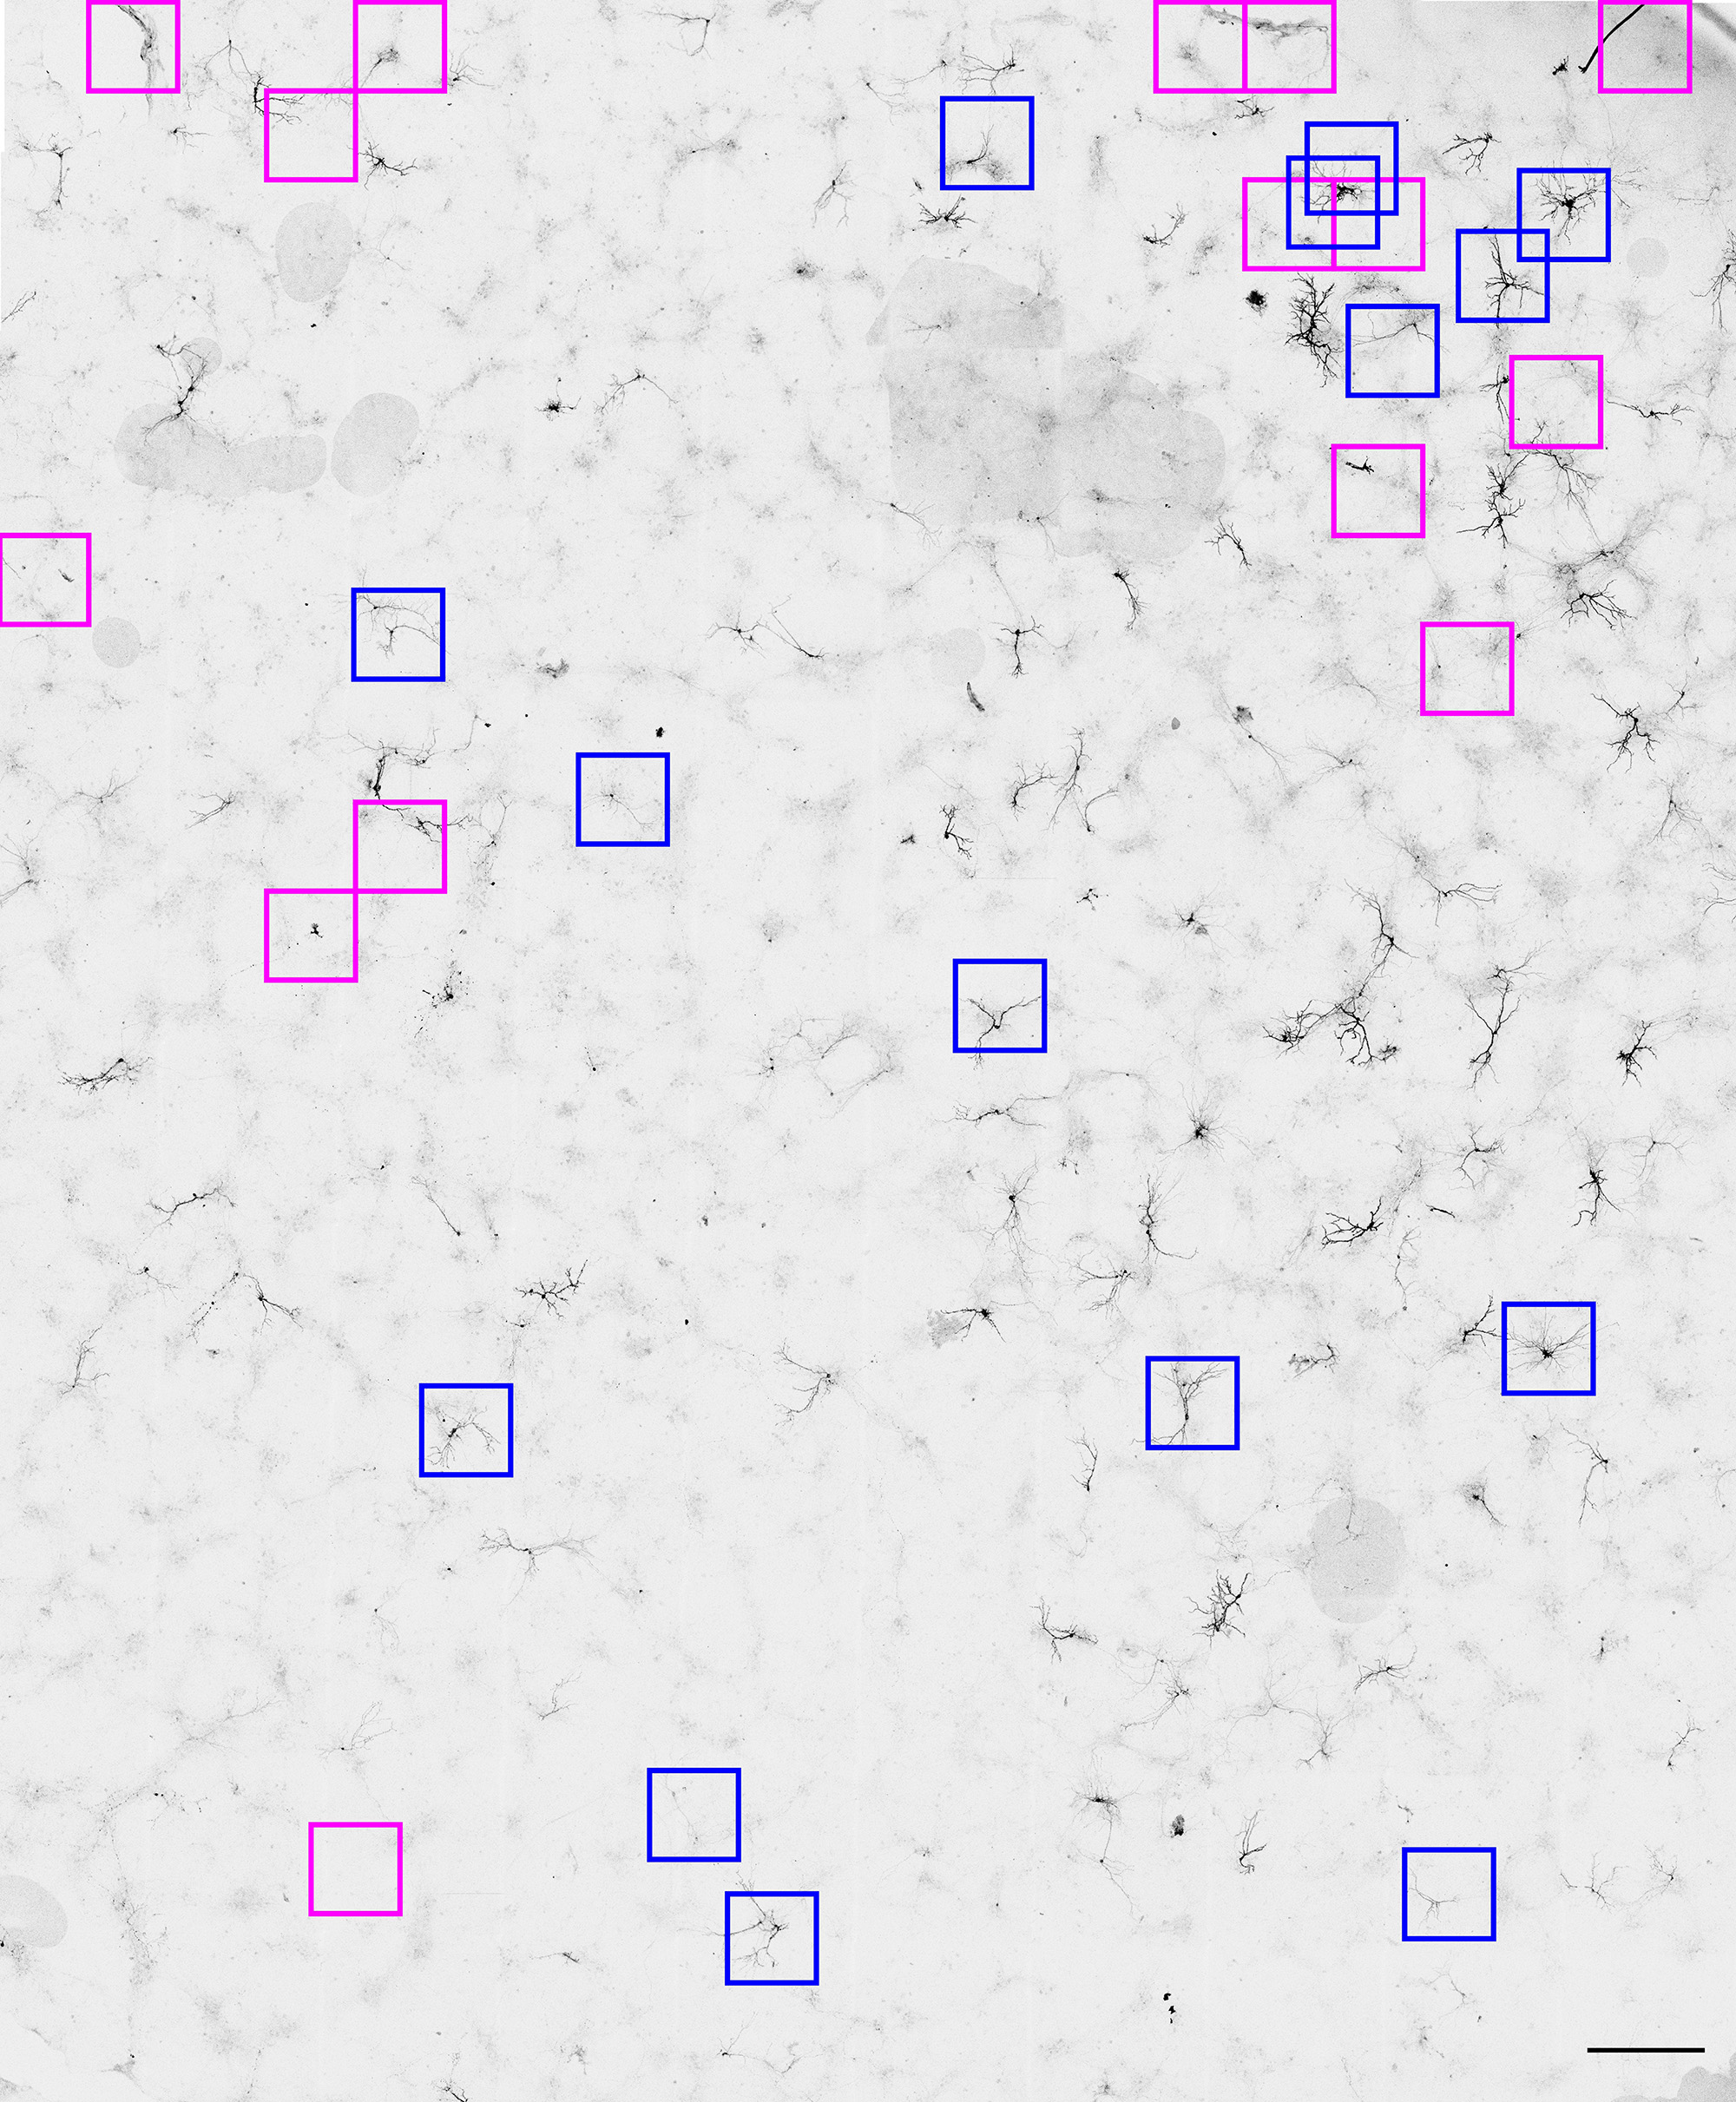
\includegraphics[width=0.55\textwidth]{fig01a}
		\vspace{-0.5em}
		\caption{Example high-content image. Scale bar: 500$\mu$m.}
		\vspace{1em}
	\end{subfigure}
	\begin{subfigure}{\textwidth}
		\centering
		\begin{tabular}{c@{\,}c@{\,}c@{\,}c@{\,}c@{}}
			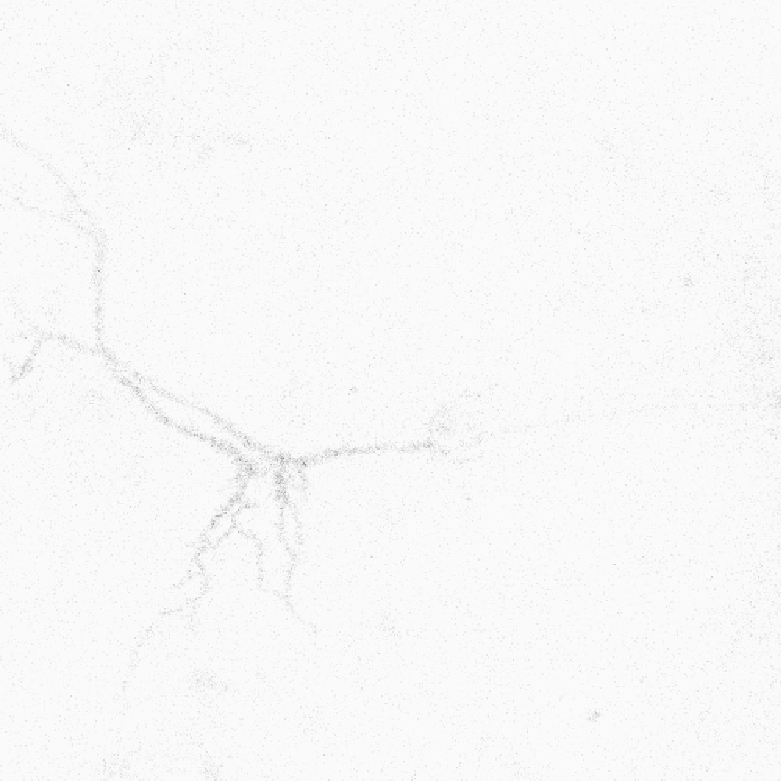
\includegraphics[width=0.1\textwidth]{fig01b01} &
			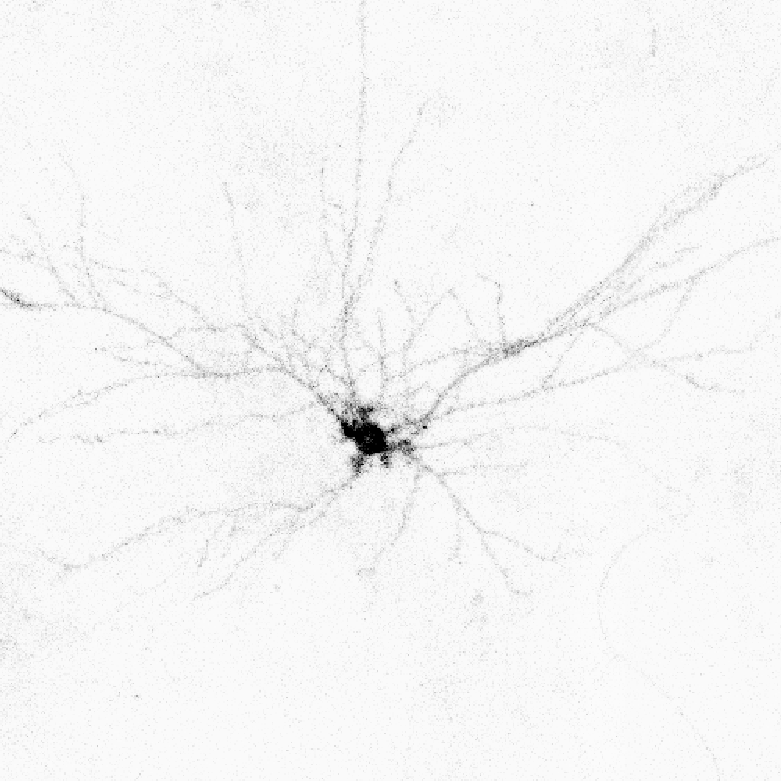
\includegraphics[width=0.1\textwidth]{fig01b02} &
			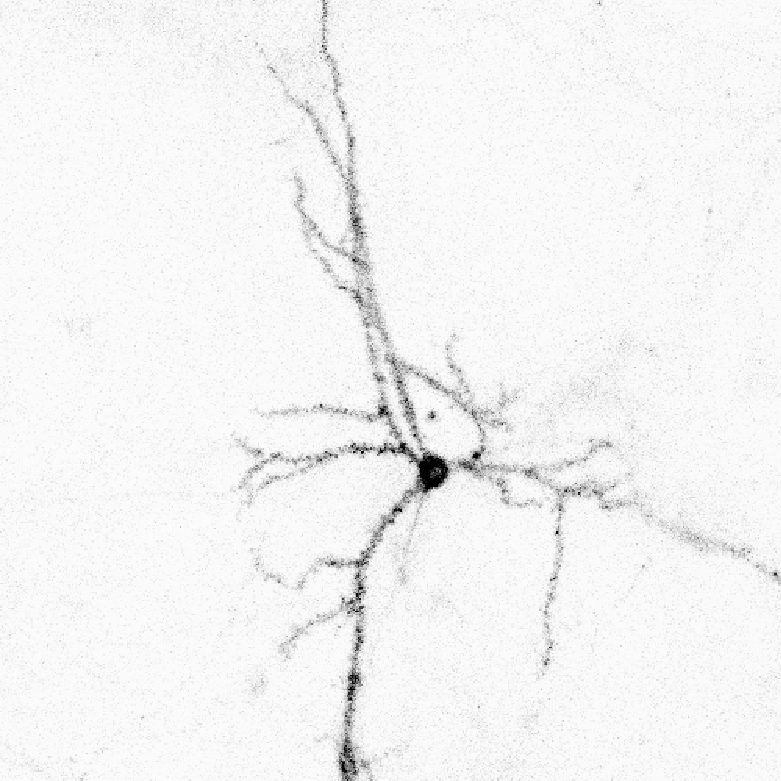
\includegraphics[width=0.1\textwidth]{fig01b03} &
			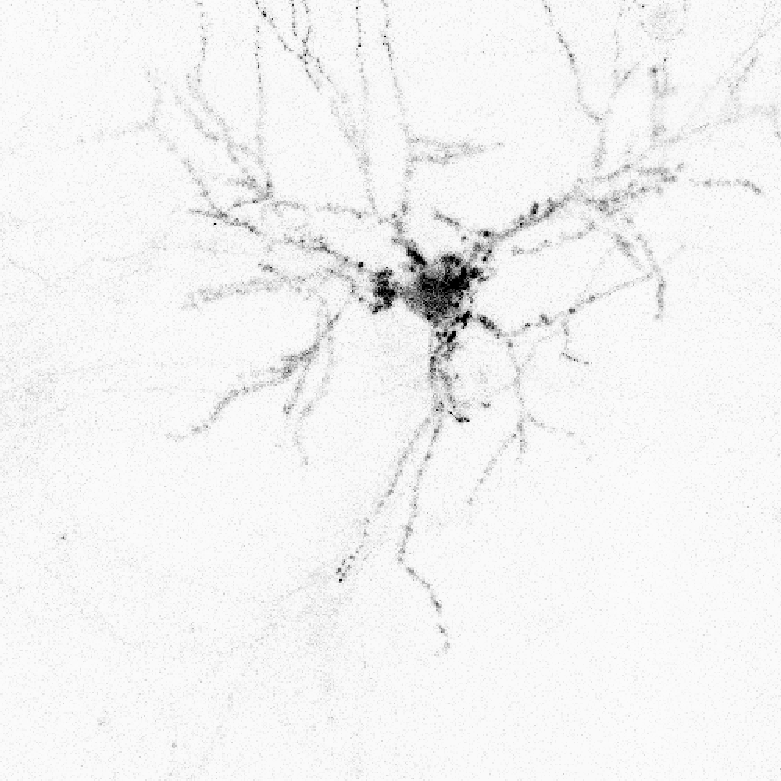
\includegraphics[width=0.1\textwidth]{fig01b04} &
			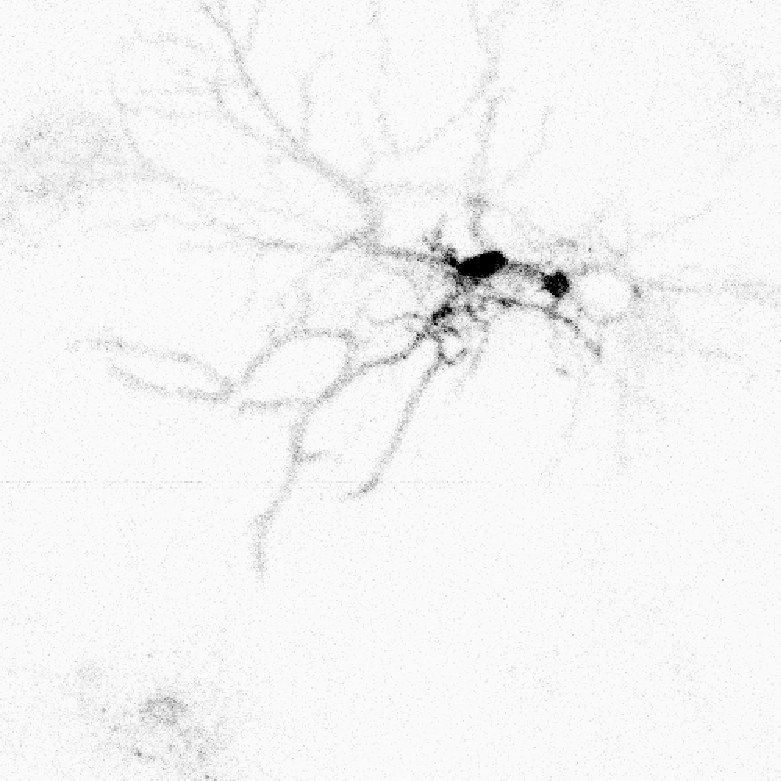
\includegraphics[width=0.1\textwidth]{fig01b05} \\
			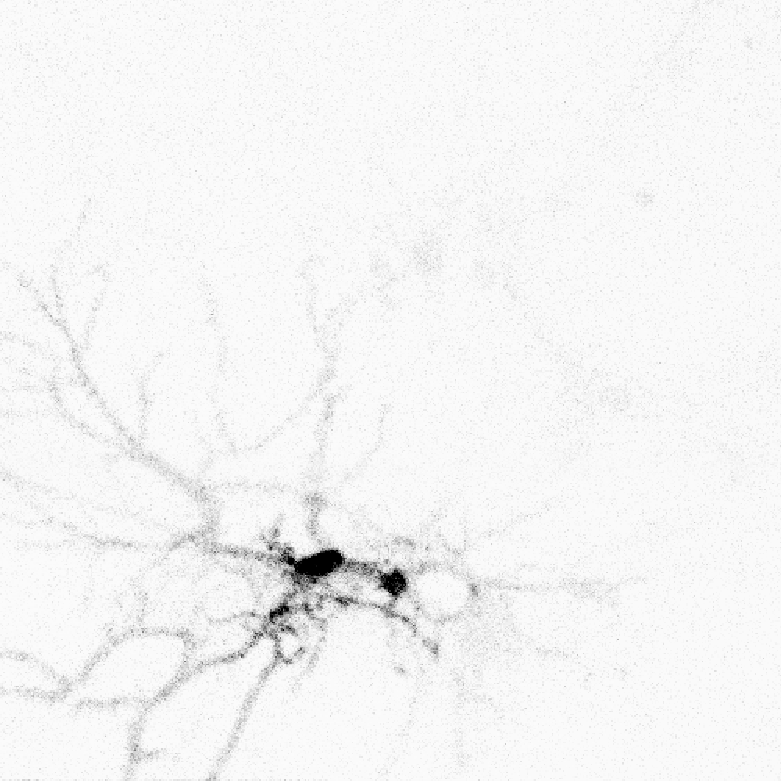
\includegraphics[width=0.1\textwidth]{fig01b06} &
			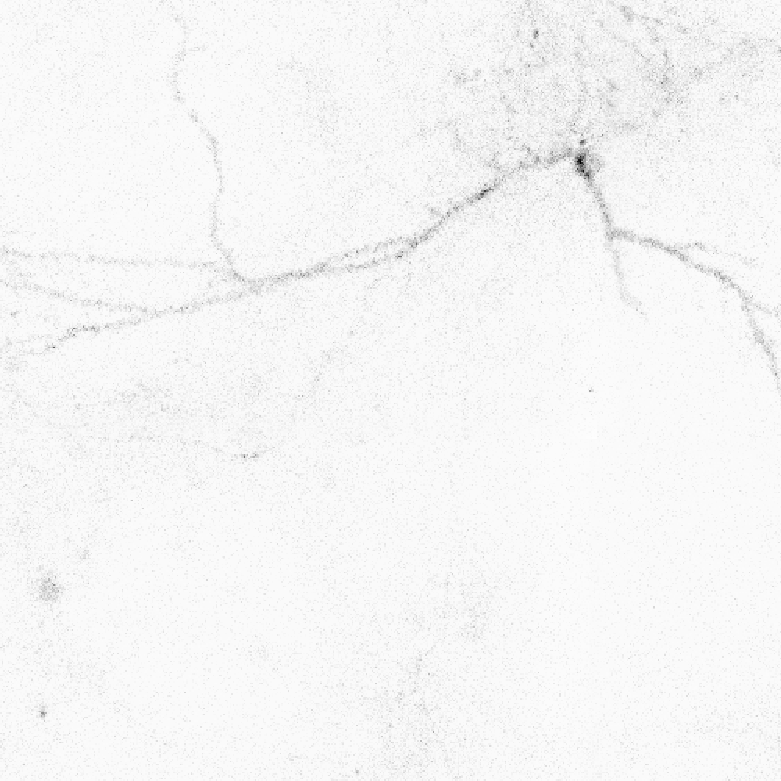
\includegraphics[width=0.1\textwidth]{fig01b07} &
			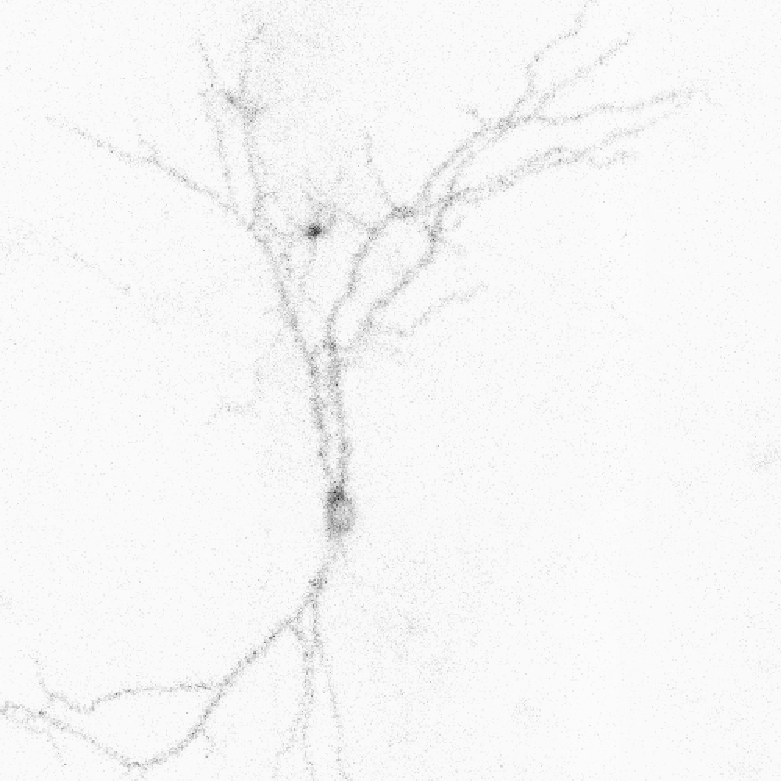
\includegraphics[width=0.1\textwidth]{fig01b08} &
			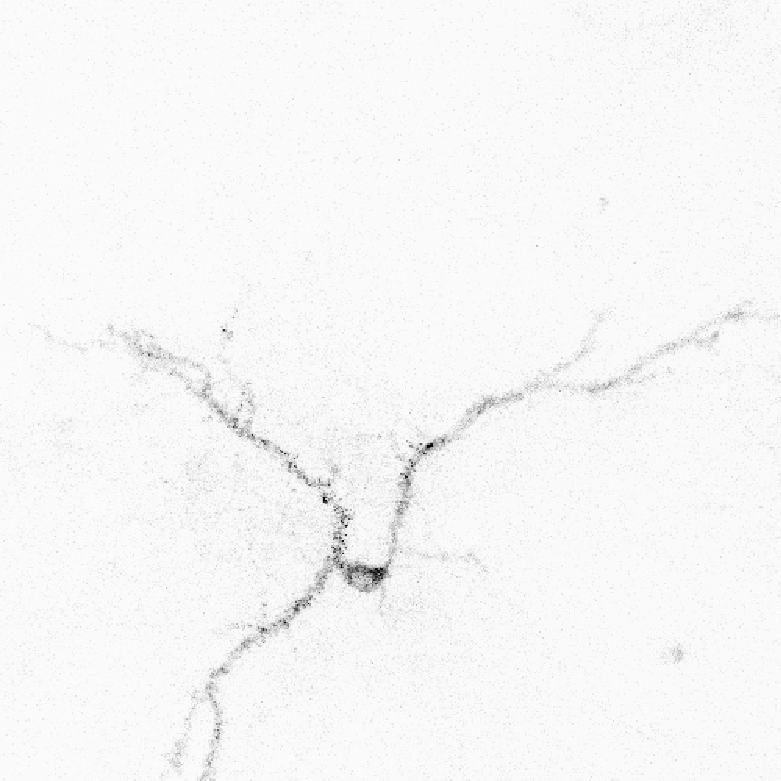
\includegraphics[width=0.1\textwidth]{fig01b09} &
			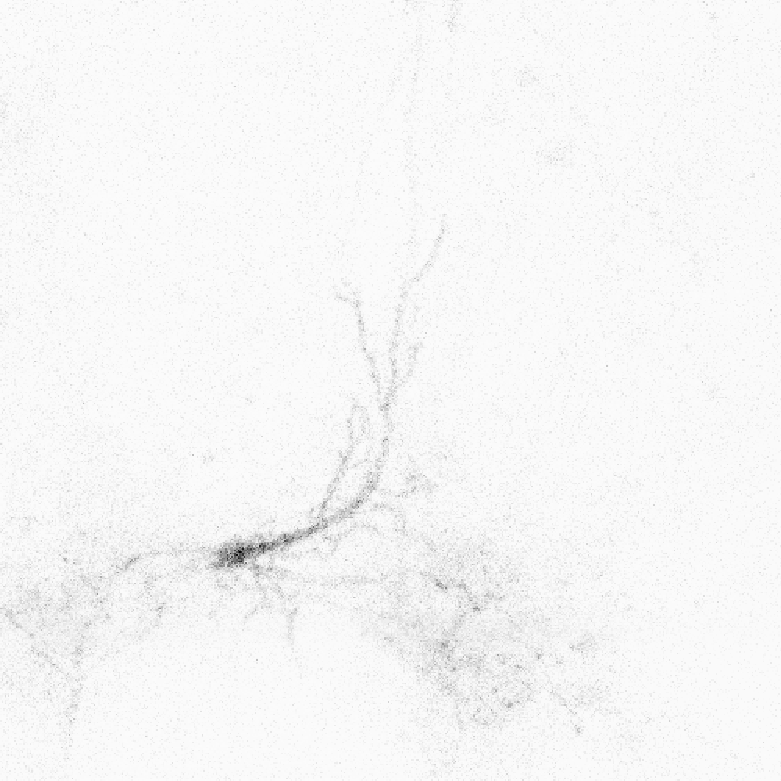
\includegraphics[width=0.1\textwidth]{fig01b10} \\
			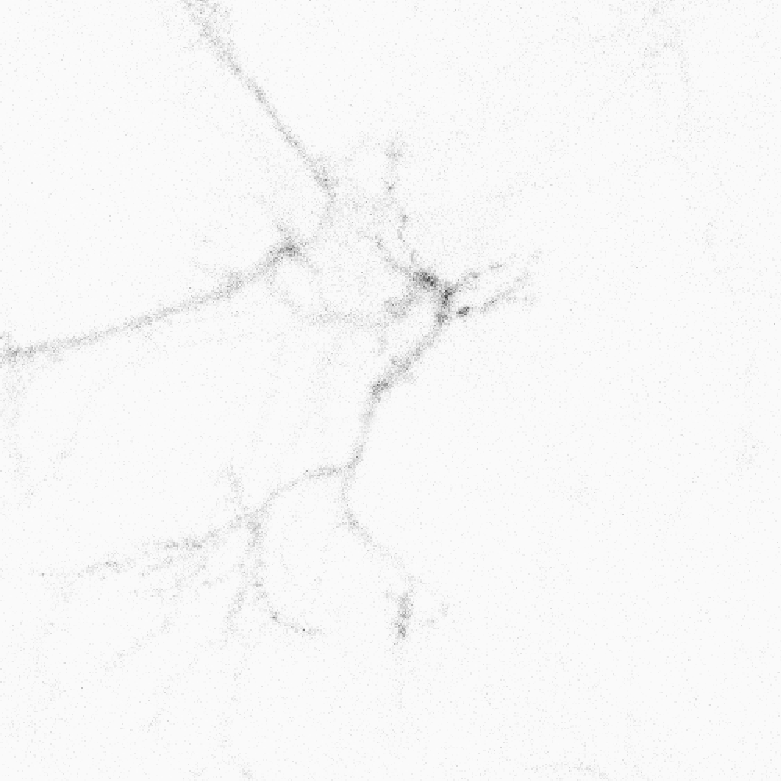
\includegraphics[width=0.1\textwidth]{fig01b11} &
			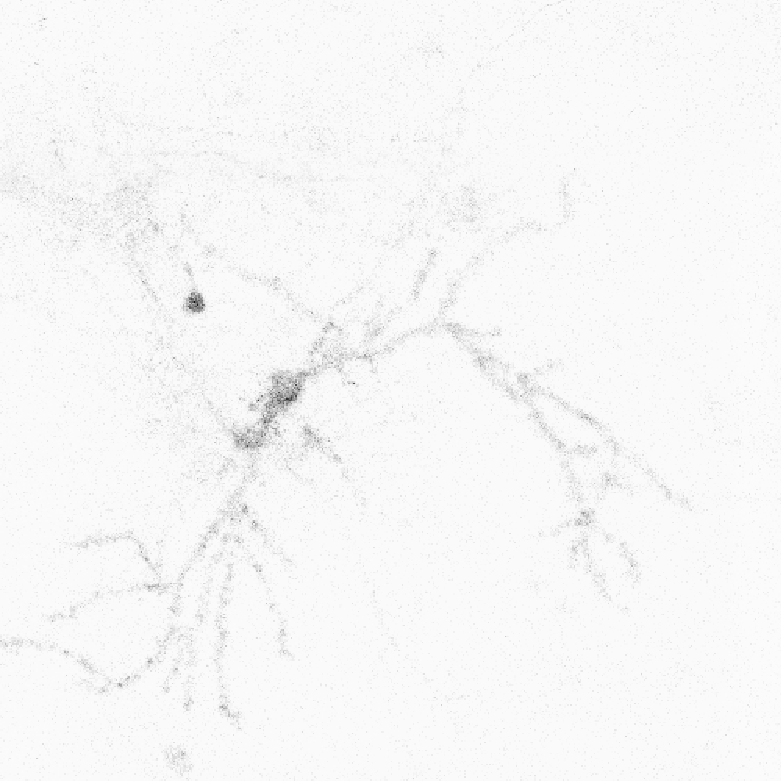
\includegraphics[width=0.1\textwidth]{fig01b12} &
			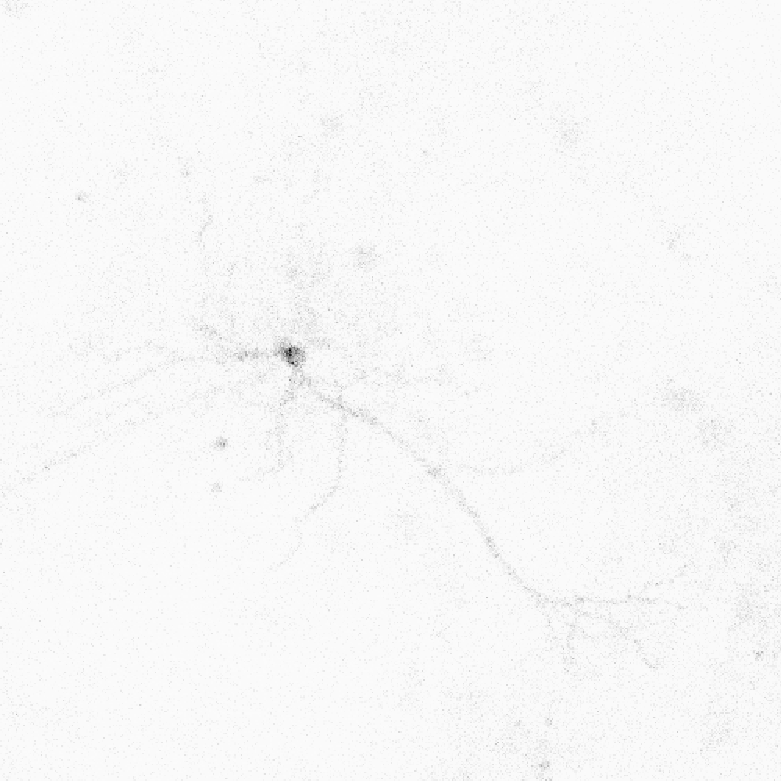
\includegraphics[width=0.1\textwidth]{fig01b13} &
			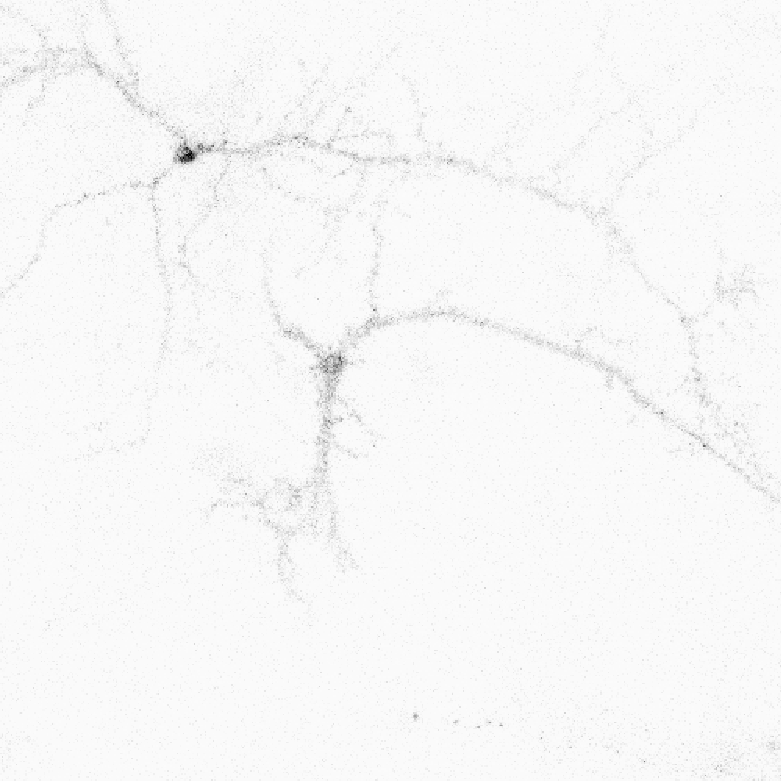
\includegraphics[width=0.1\textwidth]{fig01b14} &
			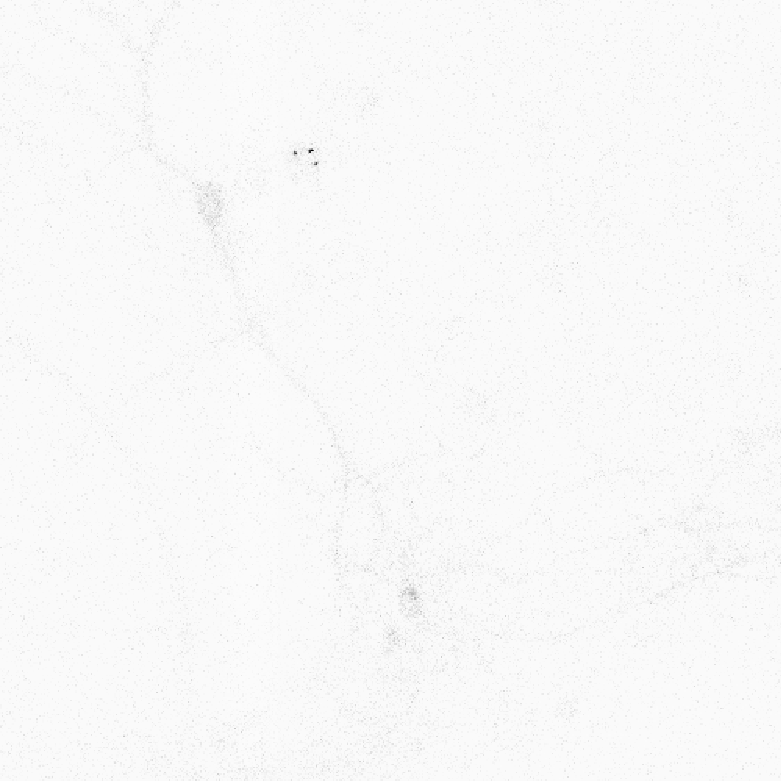
\includegraphics[width=0.1\textwidth]{fig01b15}
		\end{tabular}
	\vspace{-0.5em}
		\caption{Example patches considered as positives (blue squares).}
		\vspace{1em}
	\end{subfigure}
	\begin{subfigure}{\textwidth}
		\centering
		\begin{tabular}{c@{\,}c@{\,}c@{\,}c@{\,}c@{}}
				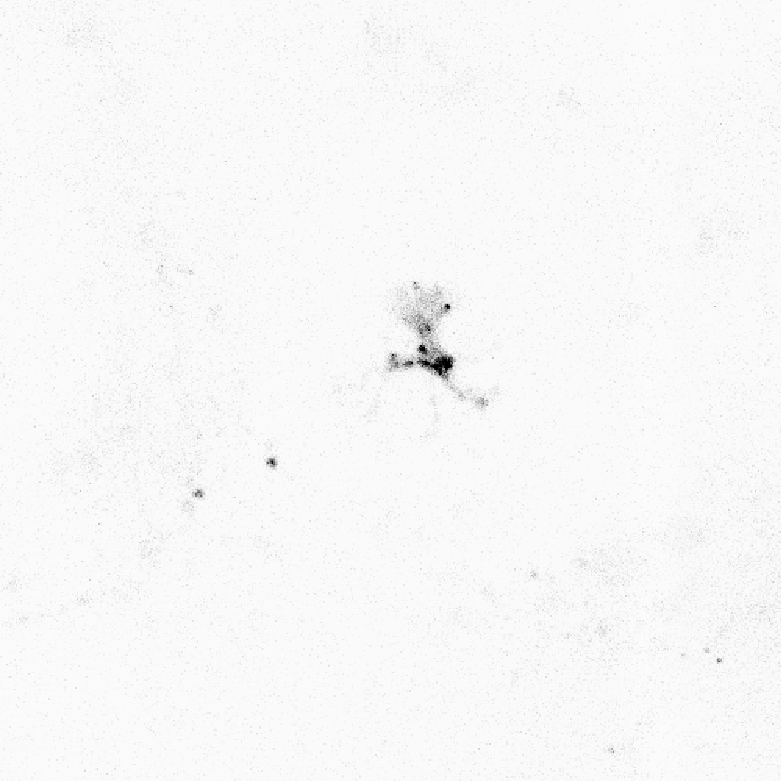
\includegraphics[width=0.1\textwidth]{fig01c01} &
				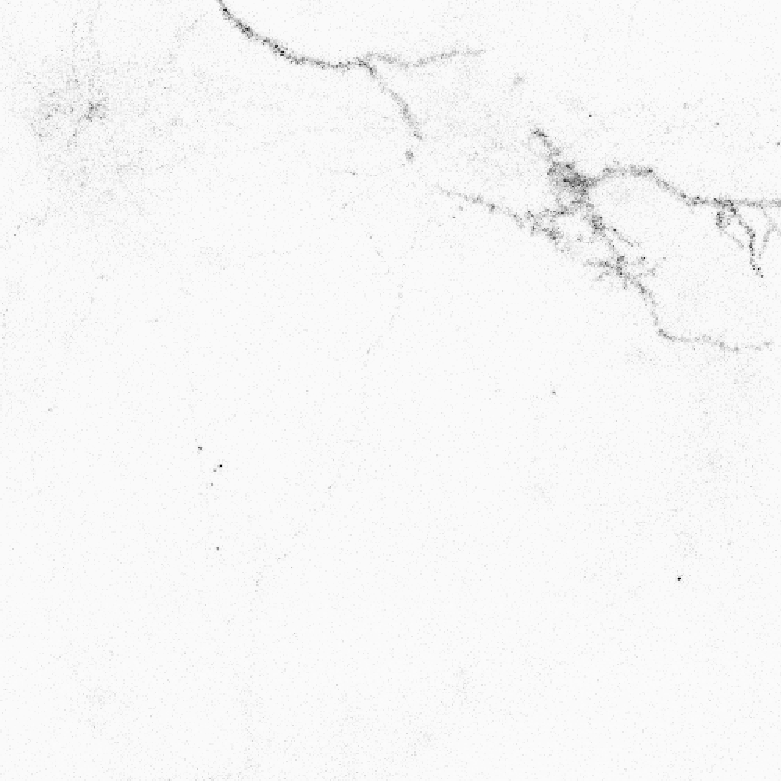
\includegraphics[width=0.1\textwidth]{fig01c02} &
				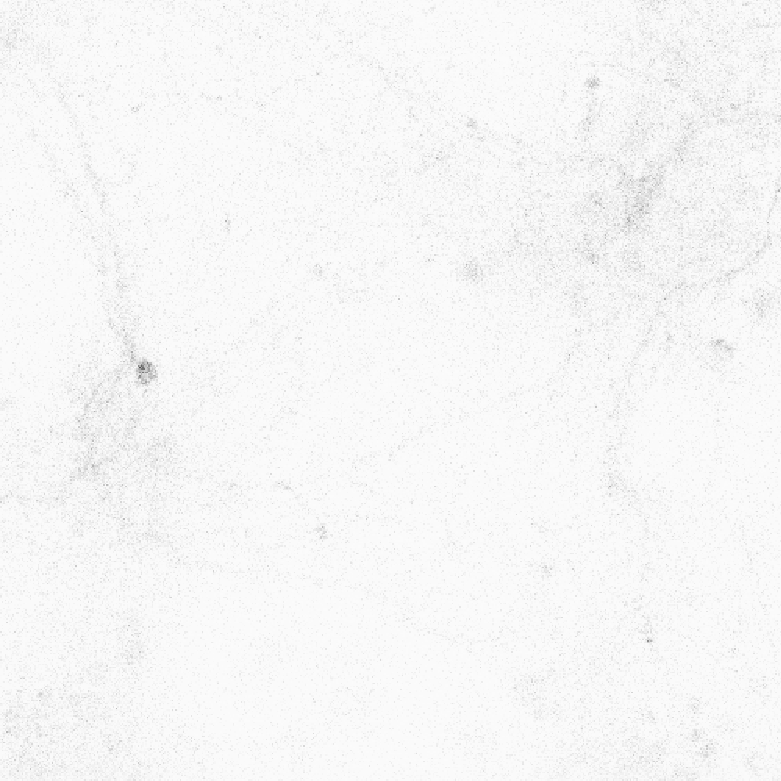
\includegraphics[width=0.1\textwidth]{fig01c03} &
				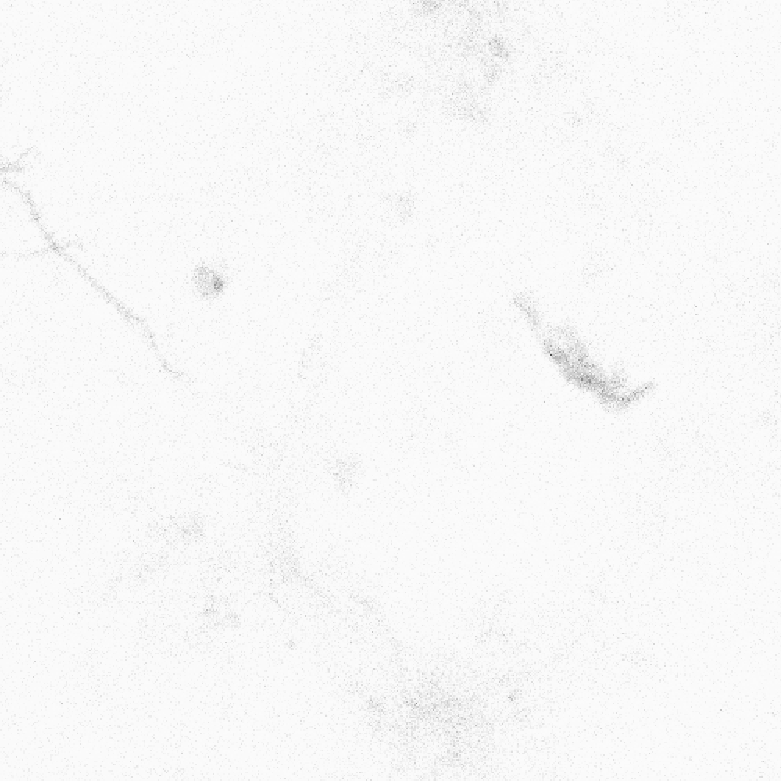
\includegraphics[width=0.1\textwidth]{fig01c04} &
				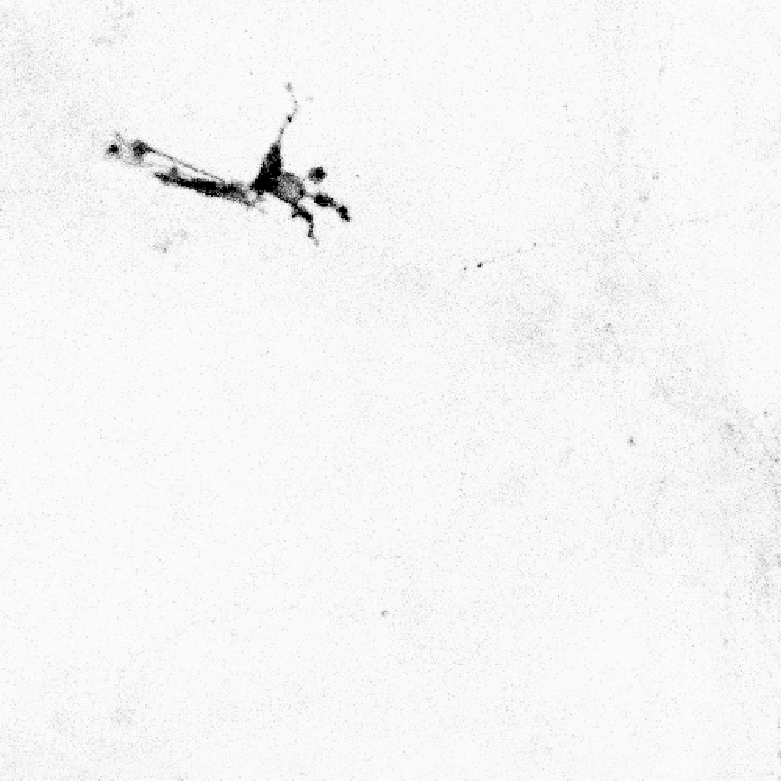
\includegraphics[width=0.1\textwidth]{fig01c05} \\
				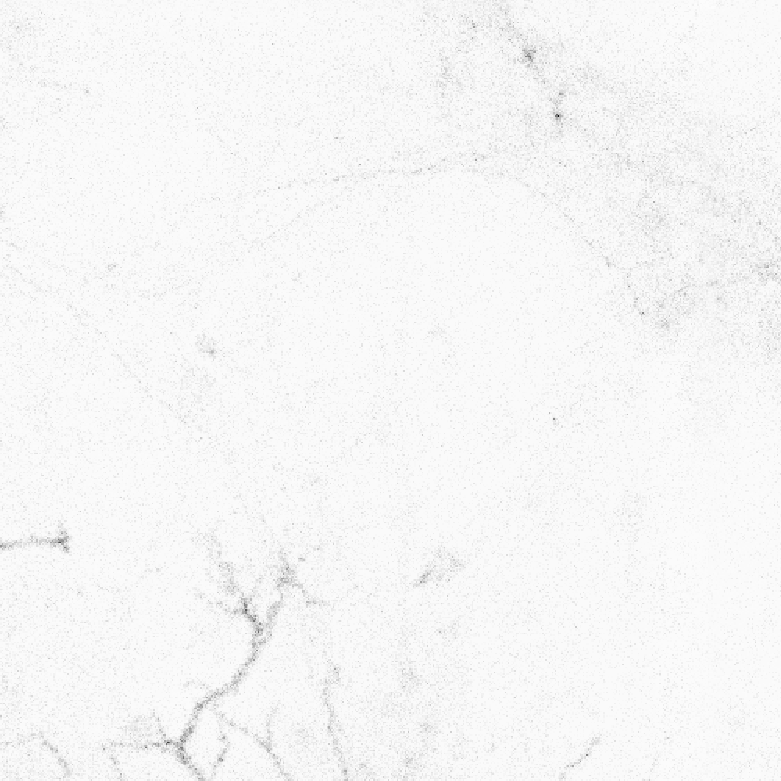
\includegraphics[width=0.1\textwidth]{fig01c06} &
				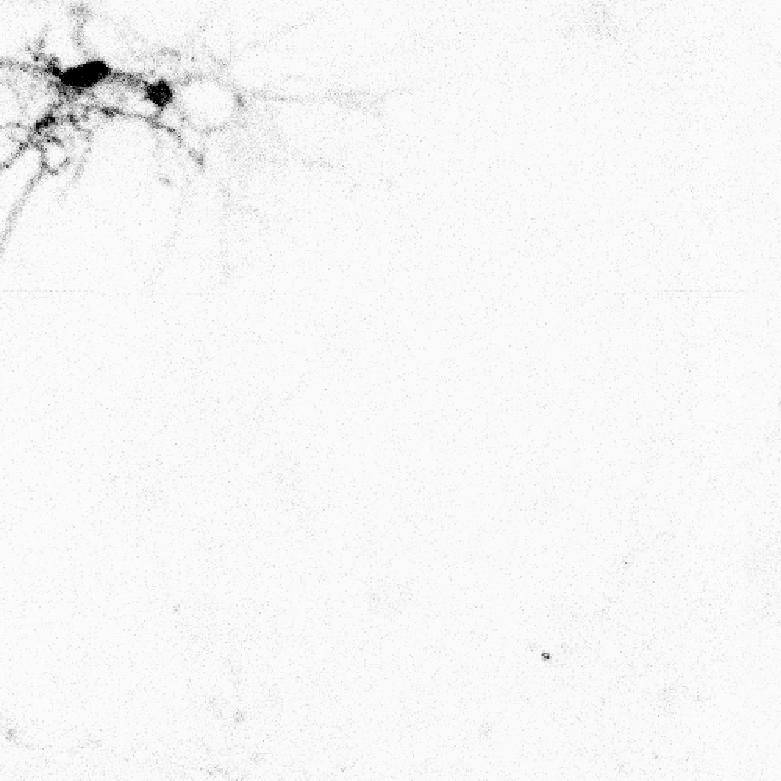
\includegraphics[width=0.1\textwidth]{fig01c07} &
				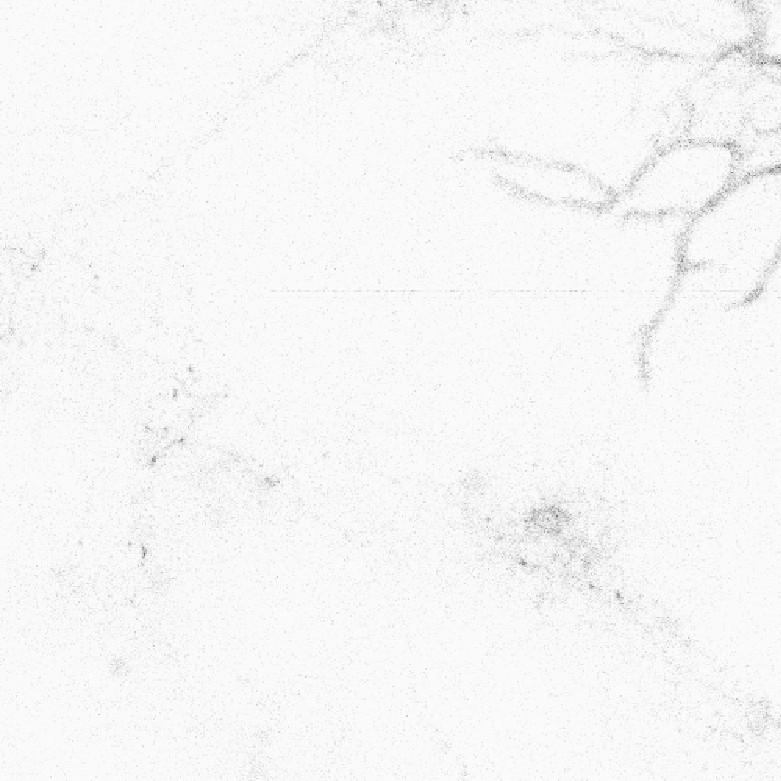
\includegraphics[width=0.1\textwidth]{fig01c08} &
				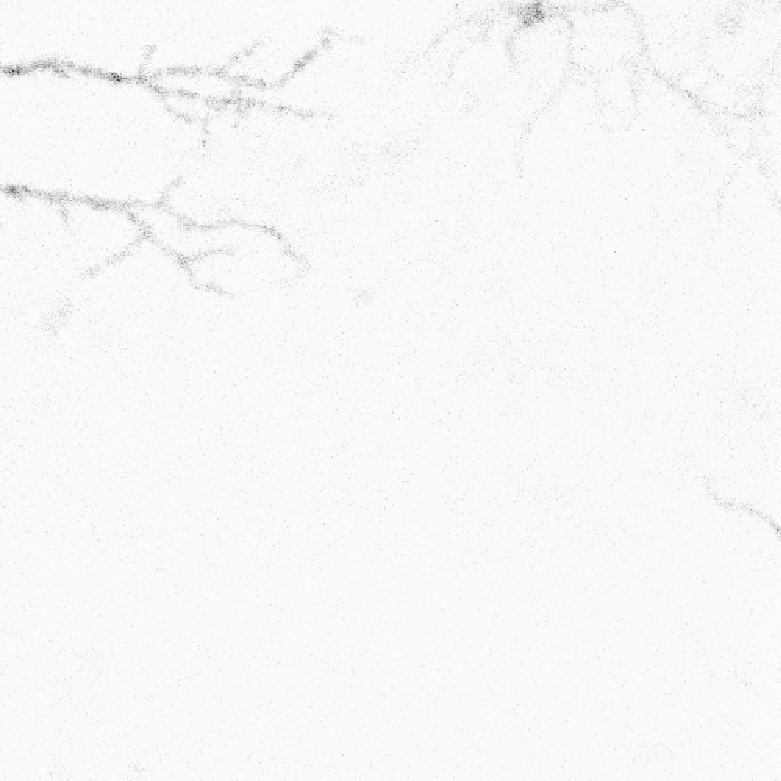
\includegraphics[width=0.1\textwidth]{fig01c09} &
				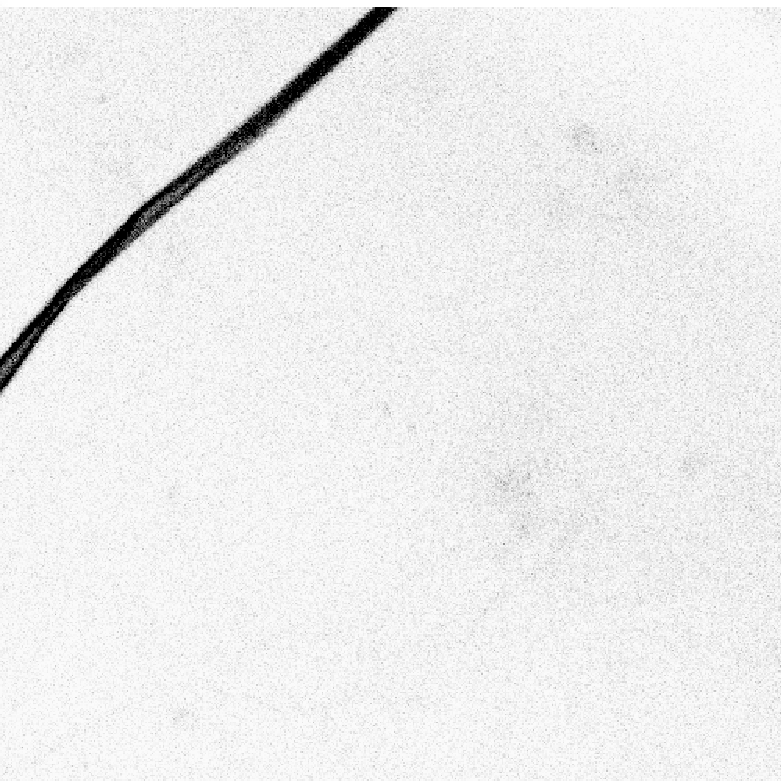
\includegraphics[width=0.1\textwidth]{fig01c10} \\
				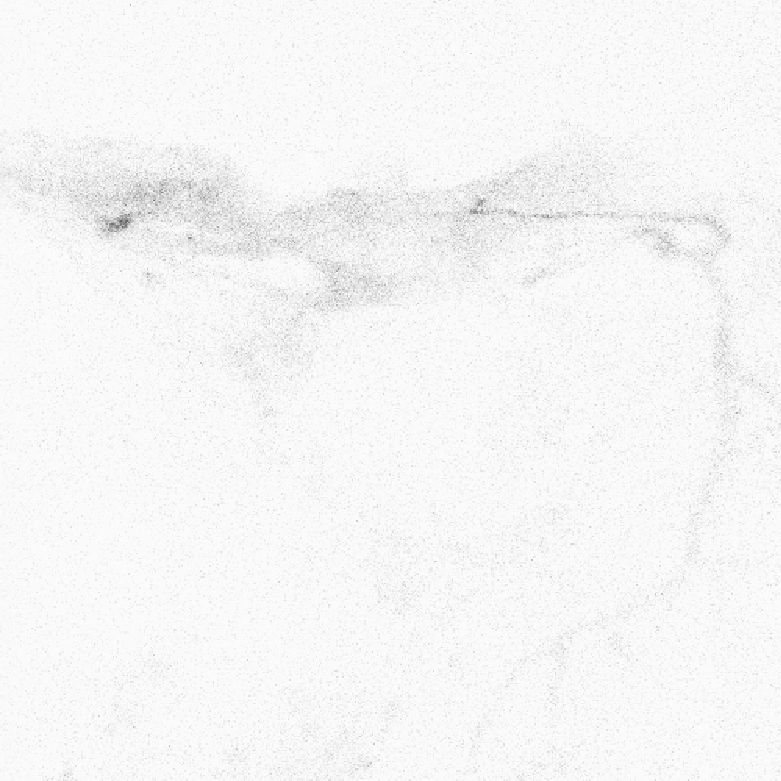
\includegraphics[width=0.1\textwidth]{fig01c11} &
				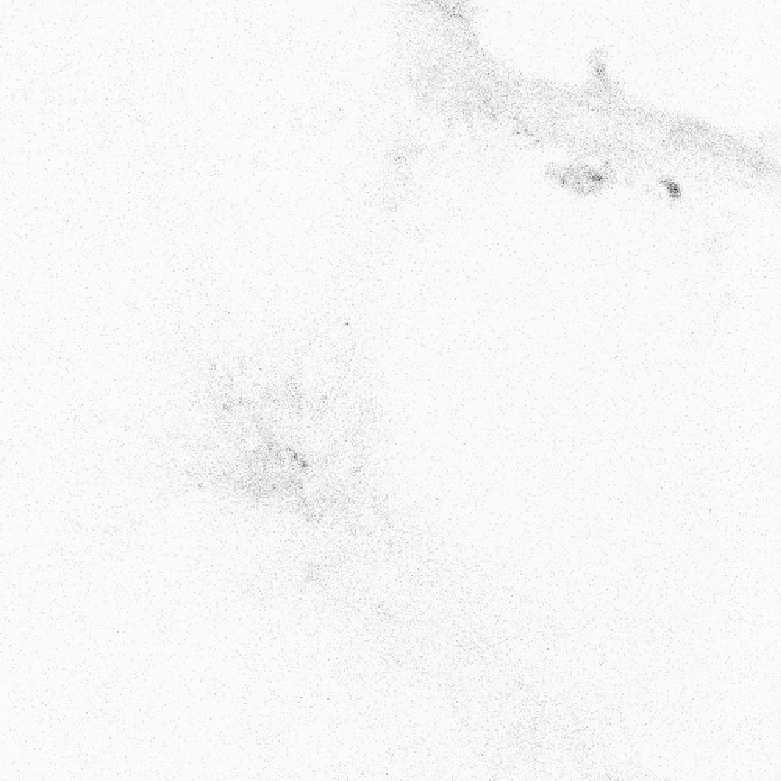
\includegraphics[width=0.1\textwidth]{fig01c12} &
				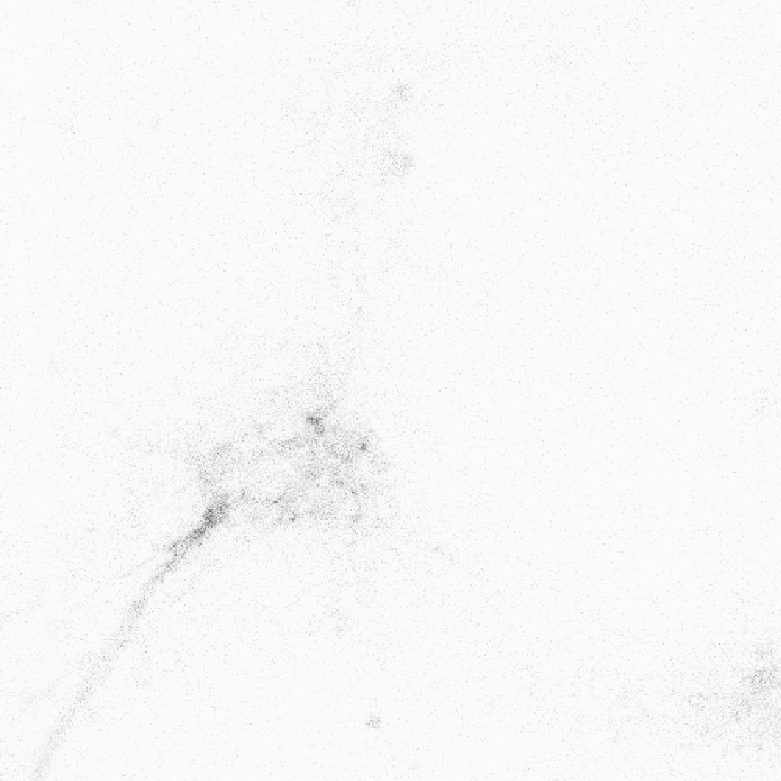
\includegraphics[width=0.1\textwidth]{fig01c13} &
				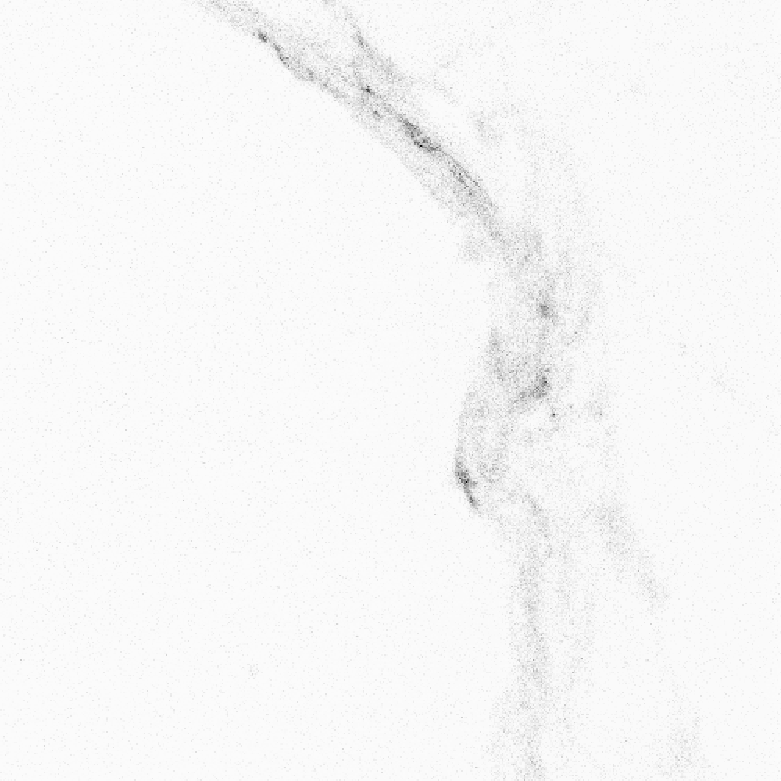
\includegraphics[width=0.1\textwidth]{fig01c14} &
				
\includegraphics[width=0.1\textwidth]{fig01c15}
			\end{tabular}
			\vspace{-0.5em}
			\caption{Example patches considered as negatives (magenta squares).}
	\end{subfigure}	
	\caption{Part of a high-content fluorescence microscopy image (a) where the blue squares highlight some example patches containing neuronal structure and the magenta squares depict some example patches containing background. These squares are enlarged in (b) and (c) for a better visualization. The intensities of the shown images are inverted compared to their originals for displaying purposes.}
	\label{fig1}%fig:example
\end{figure}

Rat hippocampal neurons were cultured and transfected with green fluorescent protein (GFP) and imaged with a Leica SP5 automated confocal fluorescence microscope using its Matrix modules and a 20$\times$ lens. The imaged neurons, coming from a part of the brain (the hippocampus) that is well known to be involved in higher functions such as learning and memory \cite{squire1992memory}, typically have a pyramidal soma with a complex dendritric tree \cite{goslin1998rat}, and their in-vivo morphological features are well conserved in culture conditions. We acquired eight two-dimensional (2D) high-content images (total size $>$1 GB), each with a size of about 10,000\,$\times$\,12,000 pixels, covering approximately 70\,mm${}^2$ of culture dish. Each image is a mosaic made up of tiles of size 1024\,$\times$\,1024 pixels, automatically acquired and stitched using the Leica Matrix module. Prior to imaging, the user has to select the desired culture area within the field of view, and the module calculates the tiles to be imaged in order to cover the chosen area, considering 10\% overlap between neighboring tiles. Each mosaic contains on the order of 40 transfected neurons (Fig.\ \ref{fig1}). Our specimens usually have about 100 neurons, but more than half of them are not or only partly imaged, as they are in different optical planes or close to the borders of the dish, making the automated detection of relevant image structures (complete neurons) as opposed to irrelevant image structures (incomplete neurons, astrocytes, and artifacts) quite challenging.

\subsubsection{Image Annotation}
\label{sec:annotation}

To obtain a reference dataset for training and testing of the machine learning methods, an expert neurobiologist manually marked all the regions of interest (ROIs) containing neurons in these images, about 400 in total. We established that relevant neurons typically cover an area of around 500 $\times$ 500 pixels in our images and therefore we fixed the ROI size to these dimensions. Using the same window size, we automatically sampled additional patches from the remaining parts of the images, containing all different types of irrelevant image structures. More specifically, to ensure evenly distributed sampling of background patches across the images, we defined a regular grid and included every patch from the grid having less than 50\% overlap with any of the neuron ROIs marked by the expert, resulting in approximately 4,500 non-neuron patches. In the sequel we refer to the neuron ROIs as `positives' and the non-neuron image patches as `negatives' (Fig.~\ref{fig1}).

\subsubsection{Dataset Balancing}
\label{sec:balanced}

Due to the sparseness of our image data, the patches of the negative class far outnumbered those of the positive class, with a ratio of approximately 10:1, resulting in an imbalanced dataset. It is well known that the performance of classification algorithms may be negatively impacted by the data being imbalanced \cite{chawla2004editorial, daskalaki2006evaluation, forman2010apples, branco2016survey}, as the algorithms may overfit the majority class and underfit the minority class, and favor the former, yielding biased results \cite{garcia2014bias, li2018adaptive}. Approaches to deal with class imbalance can roughly be divided into two categories \cite{he2008learning, Krawczyk-2016, Haixiang-2017}: data-level approaches, which modify the collection of data samples to balance the class distributions, and algorithm-level approaches, which modify the learning algorithms to alleviate their bias, for example by introducing costs to balance the importance of the different classes. Since in our case the class imbalance was substantial, and we used mostly existing algorithms and aimed to evaluate their performance without tweaking them for our application, we opted to oversample the minority class in order to obtain approximately the same number of samples in each class. To this end we employed the popular synthetic minority oversampling technique (SMOTE) \cite{Chawla:2002:SSM:1622407.1622416} of which several variants exist \cite{Saez2015, Krawczyk-2016, Gosain2017}. Specifically, for each neuron ROI marked by the expert, we also considered as potential positive samples all patches having at least 50\% overlap with that ROI (Fig.~\ref{fig:neuronROI}). However, the higher the overlap percentage of a patch, the higher the relevance of that patch, as it contains more neuron structure. Therefore, we assigned a weight to each potential patch corresponding to the overlap percentage, and taking this into account we randomly sampled from the pool of all potential patches in order to avoid bias (Fig.~\ref{fig:oversampling}). This resulted in a positive class and a negative class each consisting of approximately 4,500 samples in total.

\begin{figure}
	\centering
	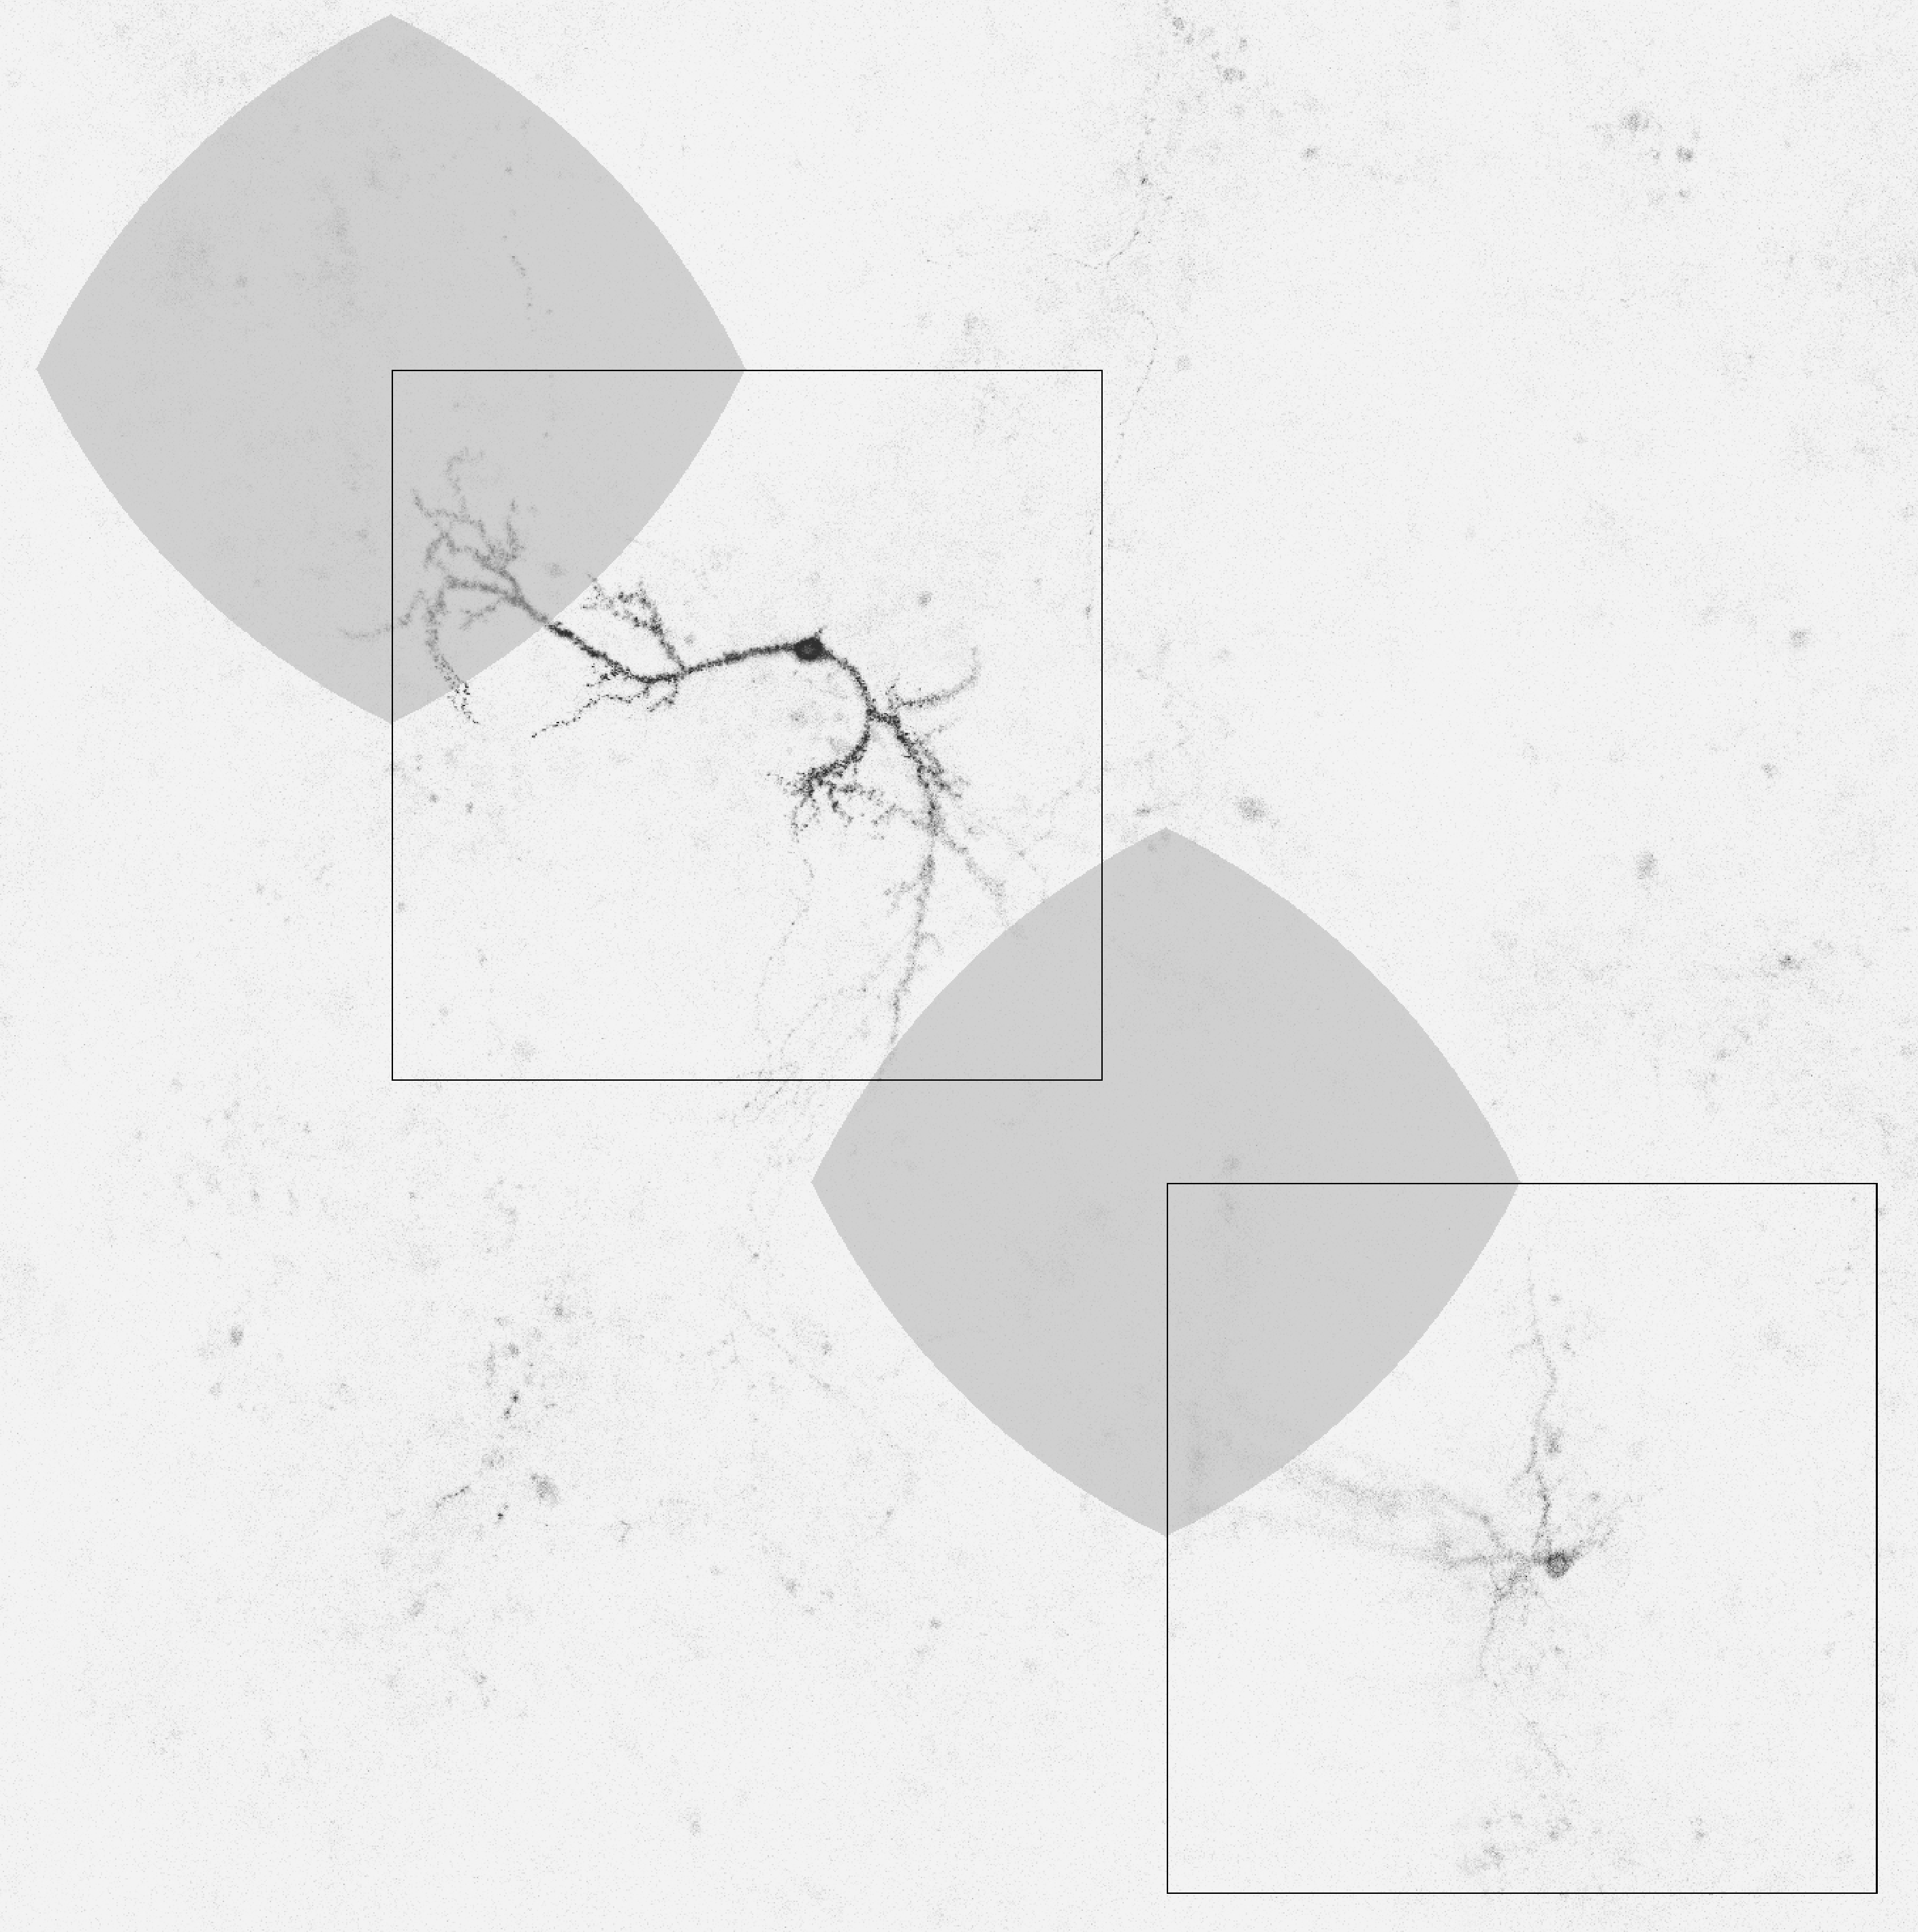
\includegraphics[width=0.2\textwidth]{fig02}
	\caption{Two example neurons with their expert-marked ROIs (black squares) and their potential alternative positive patch locations (gray regions). The latter comprise all possible top-left corner positions of patches with the same size as the given ROI and having 50\% or more area overlap with that ROI.}
	\label{fig:neuronROI}
\end{figure}

\subsection{Images Features}
\label{subsec:imageFeaturesExtraction}

To train the machine learning algorithms we used a large number of predefined features extracted from the positive and negative image patches. In this study two very comprehensive feature extraction approaches were employed: the compound hierarchy of algorithms representing morphology (CHARM) and the scale-invariant feature transform (SIFT). Here we briefly describe each of them. In the training stage of the machine learning algorithms, feature values were normalized to zero mean and unit variance per feature over the whole data set, and constant features were pruned.

\subsubsection{CHARM Features}
\label{subsubsec:wnd-chrm}

For the extraction of the CHARM features we used the open-source software library WND-CHARM \cite{shamir2008wndchrm, orlov2008wnd}, which has been successful for many pattern recognition applications in biology \cite{shamir2010pattern, uhlmann2016cp} as well as in astronomy \cite{shamir2012automatic, kuminski2014combining} and in art \cite{shamir2012computer}. It can extract a large number of generic image descriptors and also includes a classifier based on the weighted neighbor distance (WND) between feature vectors. However, since the performance of this classifier was rather limited in our initial results \cite{mata2016automatic}, we decided to explore alternative machine learning algorithms for our classification task, but using the image features calculated by this sofware library. In total we calculated 1,059 CHARM features for each positive and negative patch (recent versions of WND-CHARM can extract even more features but at an increased computational cost).



